\documentclass[11pt, addpoints, answers]{exam}

\usepackage{amsmath, amssymb}
\usepackage{xcolor}
\usepackage{tikz}
\usepackage{enumerate}
\usepackage{graphicx}
\usepackage{tabularx}
\usepackage{algorithm}
\usepackage{algpseudocode}

\newcommand{\red}[1]{\textcolor{red}{#1}}
\newcommand{\blue}[1]{\textcolor{blue}{#1}}

% For inserting code snippets.
\usepackage{listings}
\lstset{
    columns = fixed,
    basewidth = {0.5em},
    breaklines = true,
    backgroundcolor = \color{white},
    keywordstyle = \color[RGB]{40, 40, 255},
    numberstyle = \footnotesize\color{darkgray},
    commentstyle = \ttfamily\color{violet},
    basicstyle = \ttfamily,
    stringstyle = \ttfamily\color[RGB]{128, 0, 0},
    showstringspaces = false,
    language = {[11]C++},
    escapechar = \@
}
\lstnewenvironment{cpp}[1][]{\lstset{language = {[11]C++}, #1}}{}

\renewcommand{\baselinestretch}{1.15}
\setlength{\parskip}{1.25\baselineskip}

% headers, footers, titles
\newcommand{\CourseName}{CS101 Algorithms and Data Structures}
\newcommand{\HomeworkNO}{1}
\newcommand{\DueDate}{October 9, 2024}

\pagestyle{headandfoot}
\runningheadrule
\runningheader{CS101 Fall24}{Homework \HomeworkNO}{Due on: \DueDate}
\runningfooter{}{\thepage}{}

\title{
    \vspace{25pt}
    \LARGE ShanghaiTech University \\
    \bigskip
    \textbf{\CourseName} \\
    \textbf{Fall 2024}   \\
    \bigskip
    Homework \HomeworkNO
}
\author{}
\date{Due date: \DueDate, at 23:59}

% formats of questions, choices, points, etc.
\qformat{\bf\thequestion. (\totalpoints\ points) \thequestiontitle\hfill}
\pointname{'}
\CorrectChoiceEmphasis{\bf\color{blue}}
%\SolutionEmphasis{\color{blue}}

% We frequently use this font.
\newcommand{\ttt}{\texttt}
\newcommand{\bluett}[1]{\textcolor{blue}{\ttt{#1}}}

\begin{document}

\maketitle

\vspace{50pt}

\begin{enumerate}
    \item Please write your solutions in English.
    \item Submit your solutions to Gradescope.
    \item Set your FULL name to your Chinese name and your STUDENT ID correctly in Gradescope account settings.
    \item If you want to submit a handwritten version, scan it clearly. \ttt{CamScanner} is recommended.
    \item We recommend you to write in LaTeX.
    \item When submitting, match your solutions to the problems correctly.
    \item No late submission will be accepted.
    \item Violations to any of the above may result in zero points.
\end{enumerate}

\begin{questions}

\newpage
\titledquestion{Academic Integrity}

Please determine who violated academic integrity or committed plagiarism in the following situations. Tick (\(\surd\)) for the correct answers.

\begin{parts}
        %%%%%%%%%%%%%%%%%%%%%%%%%%%%%%%%%%%%%%%%%%%%%%%%%%%%%%%%%%%%%%%%%%%%%%
	% Replace `\choice' with `\CorrectChoice' on the selected choice!
	%%%%%%%%%%%%%%%%%%%%%%%%%%%%%%%%%%%%%%%%%%%%%%%%%%%%%%%%%%%%%%%%%%%%%%
	\part[1] Alice posted one of the homework questions on Stack Overflow and copied the answer from others to her homework with some trivial modifications.

	\begin{oneparcheckboxes}
		\choice Alice
		\choice Bob
		\choice Both Alice and Bob
		\choice Neither Alice nor Bob
	\end{oneparcheckboxes}

	\part[1] Alice entered the question description into ChatGPT, then slightly modified ChatGPT's response and submitted it as her own answer.

        \begin{oneparcheckboxes}
		\choice Alice
		\choice Bob
		\choice Both Alice and Bob
		\choice Neither Alice nor Bob
	\end{oneparcheckboxes}

	\part[1] Bob lent Alice his laptop to play Genshin. Alice found Bob's solution to Homework 1 on the desktop and copied it using USB drive sneakily.

	\begin{oneparcheckboxes}
		\choice Alice
		\choice Bob
		\choice Both Alice and Bob
		\choice Neither Alice nor Bob
	\end{oneparcheckboxes}

	\part[1] Alice and Bob are good friends. Alice asked if Bob could send her some code snippets so that she could have some ideas of what is going on in this programming assignment (promising, of course, not copying). Bob agreed and shared his code repository with Alice. Alice copied Bob's code, changed some variable names, and submitted the code to CS101 Online Judge.

	\begin{oneparcheckboxes}
		\choice Alice
		\choice Bob
		\choice Both Alice and Bob
		\choice Neither Alice nor Bob
	\end{oneparcheckboxes}

	\part[1] To boost efficiency and save precious time, Bob used Copilot as an assistant to write code in his programming assignments.

        \begin{oneparcheckboxes}
		\choice Alice
		\choice Bob
		\choice Both Alice and Bob
		\choice Neither Alice nor Bob
	\end{oneparcheckboxes}

	\part[1] Bob is Alice's boyfriend. In order to enhance their romantic relationship, Alice and Bob studied together in ShanghaiTech Library and collaborated on one homework question. They discussed about some algorithm using a whiteboard, without giving any exact solution.

	\begin{oneparcheckboxes}
		\choice Alice
		\choice Bob
		\choice Both Alice and Bob
		\choice Neither Alice nor Bob
	\end{oneparcheckboxes}
 
	\part[1] Alice completed the programming assignment herself on Bob's computer and accidentally submitted her code to CS101 Online Judge using Bob's account. After that, Alice and Bob resubmitted their assignments using their own accounts respectively.

	\begin{oneparcheckboxes}
		\choice Alice
		\choice Bob
		\choice Both Alice and Bob
		\choice Neither Alice nor Bob
	\end{oneparcheckboxes}
\end{parts}

\newpage
\titledquestion{Multiple Choices}

Each question has \textbf{one or more} correct answer(s). Select all the correct answer(s). For each question, you will get 0 points if you select one or more wrong answers, but you will get 1 point if you select a non-empty subset of the correct answers.

Write your answers in the following table.

%%%%%%%%%%%%%%%%%%%%%%%%%%%%%%%%%%%%%%%%%%%%%%%%%%%%%%%%%%%%%%%%%%%%%%%%%%%
% Note: The `LaTeX' way to answer a multiple-choices question is to replace `\choice'
% with `\choice', as what you did in the previous questions. However, there are 
% still many students who would like to handwrite their homework. To make TA's work 
% easier, you have to fill your selected choices in the table below, no matter whether 
% you use LaTeX or not.
%%%%%%%%%%%%%%%%%%%%%%%%%%%%%%%%%%%%%%%%%%%%%%%%%%%%%%%%%%%%%%%%%%%%%%%%%%%

\begin{table}[htbp]
	\centering
	\begin{tabular}{|p{1.7cm}|p{1.7cm}|p{1.7cm}|p{1.7cm}|p{1.7cm}|p{1.7cm}|p{1.7cm}|p{1.7cm}|p{1.7cm}|}
		\hline
		(a) & (b) & (c) & (d) & (e) & (f) \\
		\hline
		%%%%%%%%%%%%%%%%%%%%%%%%%%%%%%%%%%%%%%%%%%%%%%%%%%%%%%%%%%
		% YOUR ANSWER HERE.
		    &     &     &     &     &     \\
		%%%%%%%%%%%%%%%%%%%%%%%%%%%%%%%%%%%%%%%%%%%%%%%%%%%%%%%%%%
		\hline
	\end{tabular}
\end{table}

\begin{parts}
    \part[2] A planar graph is a graph which can be embedded in a plane i.e. you can find a way to put all vertices on the plane where the edges will not intersect with each other. Which of the statement(s) is/are correct?
    \begin{choices}
        \choice $\forall n\leq 5, K_n$ is planar. $K_n$ means the complete graph with $n$ vertices.
        \choice $K_6$ is not planar.
        \choice DAGs are planar.
        \choice A tree is planar.
        \choice Bipartite graphs are planar.
    \end{choices}

    \part[2] Given a graph $G=(V,E)$, $w(e)$ indicates the weight of edge $e$. Which of the statement(s) is/are correct?
    \begin{choices}
        \choice Both Kruskal's and Prim's algorithms can correctly find the MST even when $\exists e, w(e)<0$.
        \choice Suppose $G$ is connected and $|E| = \omega(|V|)$, $G$ has a unique MST if and only if $\forall e,e'\in E, w(e) = w(e') \Leftrightarrow e = e'$ i.e. weights of edges are distinct.
        \choice Suppose $G' = (V,E)$ is the same graph as $G$ with different weight function $v(e)$. If they share a same MST $T$, then $T$ is also the MST of $G$ with weights $u(e) = w(e) + v(e)$.
        \choice If $G$ contains multi-edges i.e. $G$ is not simple, then Kruskal's algorithm will fail but Prim's won't fail when finding MST.
    \end{choices}

	\part[2] Given a graph $G=(V,E)$, which of the following is(are) correct? 
	\begin{choices}
		\choice If $G$ is a complete graph with $4$ vertices, then the number of spanning trees of $G$ is $16$.
		\choice After Kruskal's algorithm, we choose $m$ edges, then the number of connected components of $G$ is $|V|-m$.
		\choice If $G$ is stored in adjacency matrix, then the total time complexity of Kruskal's algorithm can reach $\Theta(|V|^2+|E|\log|E|)$.
        \choice Suppose $G$ is connected and $|V| = |E|$, the maximum number of spanning trees of $G$ can reach $\Theta(|V|)$.
	\end{choices}
    
    \part[2] Let $G$ be a weighted undirected graph with positive weights where edge $e$ has weight $w_e\in \mathbb{R}^+$ for all $e \in E$. A new graph $G'$, which is a copy of $G$, and the weight of each edge $e$ in $G'$ is transformed using a function $f(w_e)$. Which of the following statements is/are true?

    \begin{choices} 
        \choice If $f(w_e) = w_e^2$, then any MST in $G$ is also an MST in $G'$.
        \choice If $f(w_e) = 2^{w_e}$, then any MST in $G$ is also an MST in $G'$.
        \choice If $f(w_e) = \frac1 {w_e}$, then any MST in $G$ is also an MST in $G'$.
        \choice If $f(w_e) = \log (w_e)$, then any MST in $G$ is also an MST in $G'$.
    \end{choices}

	\part[2] What is the number of spanning trees of following graph?

    \begin{center}
    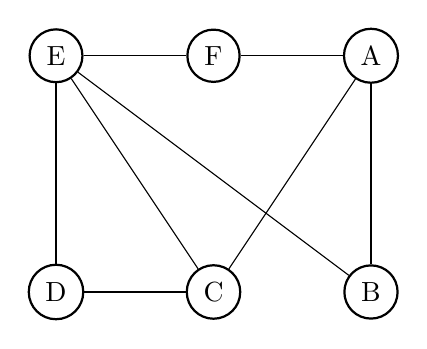
\begin{tikzpicture}
        \begin{scope}[every node/.style = {circle, thick, draw}]
            \node (A) at (2,0) {A};
            \node (B) at (2, -3) {B};
            \node (C) at (0, -3) {C};
            \node (D) at (-2, -3) {D};
            \node (E) at (-2, 0) {E};
            \node (F) at (0,0) {F};
        \end{scope}
        \begin{scope}
            \path[-] (E) edge (D);
            \path[-] (E) edge (C);
            \path[-] (E) edge (B);
            \path[-] (C) edge (D);
            \path[-] (B) edge (A);
            \path[-] (A) edge (C);
            \path[-] (A) edge (F);
            \path[-] (E) edge (F);
        \end{scope}
    \end{tikzpicture}
    \end{center}
	\begin{choices}
		\choice 32
		\choice 34
		\choice 36
		\choice 38
	\end{choices}

        \part[2] Which of the following statements are true for MST(Minimum Spanning Tree)?
        \begin{choices}
            \choice Suppose $G$ has multiple MSTs. For each minimum spanning tree $T$ of a graph $G$, there is a way to sort the edges of $G$ in Kruskal’s algorithm so that the algorithm returns $T$.
            \choice Prim's algorithm is a divide-and-conquer algorithm because it divides the graph into $S$ and $V-S$ then solve.
            \choice If we use binary heap to optimize Prim's algorithm when choosing the next edge, it will always have a better time complexity than the original algorithm on any graph.
            \choice If we add a new edge $e = (u,v)$ into a graph $G=(V,E)$ with unique MST to get a new graph $G' = (V,E\cup\{e\})$. There is at most $1$ edge difference between the MST of $G$ and $G'$.
        \end{choices}

\end{parts}


\newpage
\titledquestion{Array Representation of Linked-List}

Recall that we store a linked-list in an array to avoid memory allocation problems in the lecture. In this question, we use two arrays: \ttt{next} and \ttt{value} to implement a singly-linked-list.

The elements at each index in \ttt{next} and \ttt{value} are together to represent a node in the linked-list, where \ttt{next} represents the array index where the next node is located (\(-1\) for already reaching the tail), and \ttt{value} represents the data stoblue in the node.

\tikzstyle{listnode} = [circle, draw = black]

\begin{parts}
	\part[5] \textbf{Store a Linked-List in an Array}\par
	Fill in the table below to finish the array representation of the linked-list shown below. Fill in \(-1\) to represent the end of the linked-list.
	\begin{center}
		\begin{tikzpicture}[node distance = 2cm]z
			\node[listnode] (A) {A};
			\node[listnode, right of = A] (B) {B};
			\node[listnode, right of = B] (C) {C};
			\node[listnode, right of = C] (D) {D};
			\node[listnode, right of = D] (E) {E};
			\node[listnode, right of = E] (F) {F};
			\node[listnode, right of = F] (G) {G};
			\path[->]
                    (A) edge[bend right] node {} (C)
                    (C) edge[bend right] node {} (G)
                    (G) edge[bend right] node {} (F)
                    (F) edge[bend right] node {} (A)
                    (B) edge[bend right] node {} (E)
                    (E) edge[bend right] node {} (D);
		\end{tikzpicture}\par
		\begin{tabular}{|c|c|c|c|c|c|c|c|}
			\hline
			index & 0 & 1 & 2 & 3 & 4 & 5 & 6\\
			\hline
			\ttt{value} & A & B & C & D & E & F & G\\
			\hline
   			%%%%%%%%%%%%%%%%%%%%%%%%%%%%%%%%%%%%%%%%%%%%%%%%
			% YOUR ANSWER HERE.
            \ttt{next}&  &  &  &  &  &  & \\
            %%%%%%%%%%%%%%%%%%%%%%%%%%%%%%%%%%%%%%%%%%%%%%%%
			\hline
		\end{tabular}
	\end{center}
        \vspace{1cm}

	\part[5] \textbf{From Array to Linked-List}\par
	Here are the arrays \ttt{next} and \ttt{value}. Please draw the linked-list below represented by these two arrays.
	\begin{center}
             \vspace{1.5cm} % space above (You may remove this.)
		\begin{tikzpicture}[node distance = 2cm]
			\node[listnode] (A) {A};
			\node[listnode, right of = A] (B) {B};
			\node[listnode, right of = B] (C) {C};
			\node[listnode, right of = C] (D) {D};
			\node[listnode, right of = D] (E) {E};
			\node[listnode, right of = E] (F) {F};
			\node[listnode, right of = F] (G) {G};
            %%%%%%%%%%%%%%%%%%%%%%%%%%%%%%%%%%%%%%%%%%%%%
			% To draw an edge from X to Y, use the following command.
			%    \path[->] (X) edge node {} (Y);
			% To draw a curved edge (to avoid overlapping with the nodes):
			%    \path[->] (X) edge[bend right] node {} (Y);
			% You may remove the two `\vspace{1.5cm}'s after you have drawn the edges.
			% YOUR ANSWER HERE.
			%%%%%%%%%%%%%%%%%%%%%%%%%%%%%%%%%%%%%%%%%%%%%
                % solution

                % end solution
		\end{tikzpicture}
        \vspace{1.5cm} % space below (You may remove this.)
            
		\begin{tabular}{|c|c|c|c|c|c|c|c|c|c|c|}
			\hline
			index & 0 & 1 & 2 & 3 & 4 & 5 & 6 \\
			\hline
			\ttt{value} & A & B & C & D & E & F & G \\
			\hline
			\ttt{next} & 2 & 3 & 6 & -1 & 1 & 0 & 4 \\
			\hline
		\end{tabular}
	\end{center}
\end{parts}

\newpage
\titledquestion{Vocabulary List}

Alice is memorizing English words to enlarge her vocabulary in preparation for her approaching CET-4 test and she needs your help! Alice uses a \ttt{Node} to define a word and a linked list which contains the words that she is trying to memorize now. The structure of \ttt{Node} is as follows.

\begin{cpp}
    struct Node {
      string word;
      Node *next;
      Node(const string& _word, Node *_next)
    	  : word(_word), next(_next) {}
    };
    Node *head;
\end{cpp}

Each time she reviews her vocabulary list, she steps through the linked list starting from \ttt{head}. However, sometimes there is a word that she doesn't know, so she wants to grab the corresponding \ttt{Node} out and put it at the start of the linked list, so next time she can review it first.

For example, if the vocabulary list is 
\begin{center}
\ttt{algorithm $\rightarrow$ breath $\rightarrow$ capacity $\rightarrow$ degree}
\end{center}
and she doesn't know the word \ttt{capacity}, then she wants the list be modified to
\begin{center}
\ttt{capacity $\rightarrow$ algorithm $\rightarrow$ breath $\rightarrow$ degree}
\end{center}

\begin{parts}

    \part[6] Alice needs your help to finish her function \ttt{move\_to\_first(Node *head, Node *p)} where \ttt{head} represents the first element of her non-empty vocabulary list and she wants to move the \textbf{next} word of \ttt{p} to the first. The function returns the \textbf{new} head pointer after this process. She can guarantee that \ttt{p} points to a \ttt{Node} in the linked list, but not the last one.

    \begin{cpp}
    Node* move_to_first(Node *head, Node *p) {
        Node *to_move = p->next;
        // Write something below
        // ...
        // Write something above
    }
    \end{cpp}   

    Please help her complete the function. 

    \begin{solution}
        %%%%%%%%%%%%%%%%%%%%%%%%%%%%%%%%%%%%%%%%%%%%%%%%%%%%%%%%%%%%%
        % Replace the `\vspace*{5cm}' with your answer.
        %%%%%%%%%%%%%%%%%%%%%%%%%%%%%%%%%%%%%%%%%%%%%%%%%%%%%%%%%%%%%
        \vspace*{5cm}
    \end{solution}

    \part[4] Now Alice wants to reverse the entire list using the \ttt{move\_to\_first} function. Please help her complete the reversion function \ttt{reverse\_list(Node *head)} where \ttt{head} is the head pointer of the vocabulary list to be reversed. The function returns the \textbf{new} head pointer after this process. She can guarantee that the list is non-empty.

    \begin{cpp}
    Node* reverse_list(Node *head){
        Node *p = head;
        while(/* (1) */){
            /* (2) */ = move_to_first(/* (3) */, /* (4) */);
        }
        return head;
    }
    \end{cpp}

    Please help her complete this function by filling your code into blank (1) to (4). Each blank should be just an expression or a variable.

    \begin{solution}
        %%%%%%%%%%%%%%%%%%%%%%%%%%%%%%%%%%%%%%%%%%%%%%%%%%%%%%%%%%%%%
        % Replace the `\vspace*{5cm}' with your answer.
        %%%%%%%%%%%%%%%%%%%%%%%%%%%%%%%%%%%%%%%%%%%%%%%%%%%%%%%%%%%%%
        \vspace*{5cm}
    \end{solution}
    

    
\end{parts}


\newpage
\titledquestion{Postfix Expression}
Reverse Polish notation (RPN) is a mathematical notation in which operators follow their operands. Using a stack, we can evaluate postfix notation equations easily.

A postfix expression (Reverse-Polish Notation) with single-digit operands is shown below: (where $\hat\ $ is the exponentiation operator)\\
    $$\mathtt{8\ 2\ 3\ \hat \ /\ 2\ 3\ *\ +\ 5\ 1\ *\ -}$$
    
\begin{parts}
    \part[1] What's the in-fix expression of the expression above?
    \begin{solution}
        \vspace*{1cm}
    \end{solution}
    
    \part[4] The changing of the stack to calculate the final result is:
    \begin{table}[h]
        \centering
        \begin{tabular}{|p{0.25cm}|p{0.1cm}|p{0.25cm}|p{0.1cm}|p{0.25cm}|p{0.1cm}|p{0.25cm}|p{0.1cm}|p{0.25cm}|p{0.1cm}|p{0.25cm}|p{0.1cm}|p{0.25cm}|p{0.1cm}|p{0.25cm}|p{0.1cm}|p{0.25cm}|p{0.1cm}|p{0.25cm}|p{0.1cm}|p{0.25cm}|p{0.1cm}|p{0.25cm}|p{0.1cm}|p{0.25cm}|}
            \cline{1-1} \cline{3-3} \cline{5-5} \cline{7-7} \cline{9-9} \cline{11-11} \cline{13-13} \cline{15-15} \cline{17-17} \cline{19-19} \cline{21-21} \cline{23-23} \cline{25-25}
             &  &  &  &  &  &  &  &  &  &  &  &  &  &  &  &  &  &  &  &  &  &  &  &  \\ \cline{1-1} \cline{3-3} \cline{5-5} \cline{7-7} \cline{9-9} \cline{11-11} \cline{13-13} \cline{15-15} \cline{17-17} \cline{19-19} \cline{21-21} \cline{23-23} \cline{25-25}
             &  &  &  &  &  &  &  &  &  &  &  &  &  &  &  &  &  &  &  &  &  &  &  &  \\ \cline{1-1} \cline{3-3} \cline{5-5} \cline{7-7} \cline{9-9} \cline{11-11} \cline{13-13} \cline{15-15} \cline{17-17} \cline{19-19} \cline{21-21} \cline{23-23} \cline{25-25}
             &  &  &  &  &  &  &  &  &  &  &  &  &  &  &  &  &  &  &  &  &  &  &  &  \\ \cline{1-1} \cline{3-3} \cline{5-5} \cline{7-7} \cline{9-9} \cline{11-11} \cline{13-13} \cline{15-15} \cline{17-17} \cline{19-19} \cline{21-21} \cline{23-23} \cline{25-25}
             &  &  &  &  &  &  &  &  &  &  &  &  &  &  &  &  &  &  &  &  &  &  &  &  \\ \cline{1-1} \cline{3-3} \cline{5-5} \cline{7-7} \cline{9-9} \cline{11-11} \cline{13-13} \cline{15-15} \cline{17-17} \cline{19-19} \cline{21-21} \cline{23-23} \cline{25-25}
        \end{tabular}
    \end{table}

    \part[3] Try to convert the following in-fix expression into post-fix expression: (You don't need to calculate them)

    (1) $ 1*2+3 $
    \begin{solution}
        \vspace*{1cm}
    \end{solution}
    (2) $ 1 + 2*3 + (4 * 5 + 6) * 7 $
    \begin{solution}
        \vspace*{1cm}
    \end{solution}
    (3) $ 1 + (2*3  \hat\   4) /(5+6)+7$
    \begin{solution}
        \vspace*{1cm}
    \end{solution}

    \part[2] Please judge whether the following post-fix expression is legal. Tick (\(\surd\)) for the legal expressions.
    
    \begin{oneparcheckboxes}
        \choice $ 1\ 2\ *\ +\ 3\ 5\ +\ $ 
        \choice $ 4\ 5\ 6\ /\ *\ 1\ /\ $ 
        \choice $ 1\ +\ 2\ -\ 3\ +\ 4\ $ 
        \choice $ 7\ 8\ 9\ 1\ +\ -\ *\ $ 
    \end{oneparcheckboxes}
\end{parts}

\newpage
\titledquestion{Compare and Prove}

For each pair of functions $f(n)$ and $g(n)$, give your answers whether $f(n) = o(g(n))$, $f(n) = \omega(g(n))$ or $f(n) = \Theta(g(n))$.  Give a \textbf{proof} of your answer. 

\textbf{Note 1}: Give your answer in the most precise form. 

\textbf{Note 2}: You'd better try to prove them by calculating limits.

\begin{parts}
    \part[3] $f(n) = {1.01}^n$ and $g(n) = n^{10}$
    \begin{solution}
        \vspace*{16cm}
    \end{solution}

    \newpage
    \part[4] $f(n) = \log(n!)$ and $g(n) = \log(n^n)$
    \begin{solution}
        \vspace*{16cm}
    \end{solution}
    
    \newpage
    \part[4] $f(n) = n^{1+\varepsilon}, \varepsilon\in \mathbb{R}^+$ and $g(n) = n(\log n)^k, k \in \mathbb{Z}^+$
    \begin{solution}
        \vspace*{16cm}
    \end{solution}
\end{parts}

\newpage
\titledquestion{Problem Analysis}

Consider the following basic problem:

You're given an array $A$ consisting of n integers $A[1], A[2], ..., A[n]$. You'd like to output a two-dimensional $n$-by-$n$ array $B$ in which $B[i, j]$ (for $i < j$) contains the sum of array entries $A[i]$ through $A[j]$ -- that is, the sum $A[i] + A[i+1] + ... + A[j]$. (the value of array entry $B[i, j]$ is left unspecified whenever $i \ge j$.)

Here's the pseudocode of a simple algorithm to solve this problem. (Initially $B[i,j]=0$ for all valid $i,j$)

\begin{algorithmic}[1]
\For{$i = 1$ \textbf{to} $n$}
    \For{$j = i+1$ \textbf{to} $n$}
        \For{$k = i$ \textbf{to} $j$}
            \State $B[i,j]\gets B[i,j] + A[k]$
        \EndFor
    \EndFor
\EndFor
\end{algorithmic}

For the following questions,
\begin{itemize}
    \item Define $T(n)$ as the total running time of the algorithm.
    \item Suppose each operation like $B[i,j]\gets B[i,j] + A[k]$ costs a constant time $c$.
    \item Ignore the time that \lstinline|for| loop iterations take.
\end{itemize}
\begin{parts}
    \part[1] Give out a function $f$ satisfying that the running time of the algorithm is $\Theta(f(n))$. That is, $T(n)=\Theta($\fillin[]$)$. (Give your answer in the most simplified form.)

    \part[3] For this function chosen \( f \), show that the running time of the algorithm on an input of size \( n \) is upper bounded by \( f(n) \). That is, prove $T(n)=O(f(n))$.
    \begin{solution}
        \vspace*{7cm}
    \end{solution}

    \part[4] For the same function \( f \), show that the running time of the algorithm on an input of size \( n \) is also lower bounded by \( f(n) \). That is, prove $T(n)=\Omega(f(n))$.
    \begin{solution}
        \vspace*{7cm}
    \end{solution}

    \part[3] Although the algorithm you just analyzed is the most natural way to solve the problem---after all, it just iterates through the relevant entries of the array \( B \), filling in a value for each---it contains some highly unnecessary sources of inefficiency. Give a different algorithm to solve the problem, with an asymptotically better running time. In other words, you should design another algorithm with running time \( \Theta(g(n)) \), where \( \lim\limits_{n \to \infty} \frac{g(n)}{f(n)} = 0 \).
    
    Just write the pseudocode below.
    \begin{solution}
        \vspace*{7cm}
    \end{solution}
\end{parts}

\end{questions}

\end{document}